\documentclass[a4paper]{article}

%% Language and font encodings
\usepackage[english]{babel}
\usepackage[utf8x]{inputenc}
\usepackage[T1]{fontenc}

%% Sets page size and margins
\usepackage[a4paper,top=3cm,bottom=2cm,left=3cm,right=3cm,marginparwidth=1.75cm]{geometry}

%% Useful packages
\usepackage{amsmath}
\usepackage{graphicx}
\graphicspath{ {images/} }

\usepackage[colorlinks=true, allcolors=blue]{hyperref}

\title{Assignment 5 - User Stories and Set-up Assignment (USSA)}
\author{ by Group 3 - Plant-Id \\* \\* Team Members: \\* Ethan Ahuja - ahujae \\* Ethan Patterson - patteret \\* James Barry - barryj \\* Evan Brass - brassev \\* \\* Customers: \\* Ethan Ahuja - ahujae \\* Ethan Patterson - patteret}
\begin{document}
\maketitle
\pagebreak
\tableofcontents
\pagebreak
\section{GitHub Link}
Due to past submission issues, we have chosen to also include our GitHub URL here in the document: \url{https://github.com/barryjosu/CS361-001-W2018/tree/plant-id-assignment-5}
\section{User Stories}
\subsection{Story 1 - 20 Questions}
A user would like to identify a plant, so they can open the app, press the "20 Questions" button, and answer a series of questions to identify the plant.
\subsection{Story 2 - Photo Identification}
A user would like to identify a plant with a picture, so they can open the app, press the "Photo Identification" button, and submit a photo of the plant for the app's neural network to identify.
\subsection{Story 3 - Incorrect Identification}
The system incorrectly identifies a plant through the question process, so the user can submit a picture of the plant and send geotracking information to the server for admins to correct the error.
\subsection{Story 4 - Correct Identification}
The system correctly identifies a plant, so the user can send geotracking information of where they found it to the database for plant mapping. They can also view information about the plant, including its name, edibility, and if it is save to touch
\subsection{Story 5 - Settings}
As a user, I would like to change the behavior of the app.  I would, click the "Help" button on the main menu and then the "Settings" button on the "Help" menu and edit them. Some options I want to be able to control are: whether or not my geolocation is default set to be included when I report finding a plant and manually fetch updates to the local plants database.
\subsection{Story 6 - Learn More}
The user would like to know more about the application, so they can click the "How It Works" button on the "Help" menu to view information about how the app identifies plants.
\subsection{Story 7 - Send Feedback}
The user would like to send in feedback, so they can click the "Contact Us" button under the "Help" menu to type feedback and send it to the developers. 
\subsection{Story 8 - Create an Account}
A user would like to create an account for keeping track of their plant findings, so they can press the "Create an Account" button on the main menu. They will create a username and password for logging into their account. Any findings they make will automatically be assigned to their account.
\subsection{Story 9 - Become a Botanist}
A user would like to have a botanist account on the system, giving them access to information on the database. They can press the "Become a Botanist" button on the "Help" menu to go through a process of submitting their certification to the developers for verification. They will be given login information for their botanist account.
\subsection{Story 10 - Welcome Screen}
The user will receive a "Welcome" screen the first time they launch the application, welcoming them and giving them a short explanation of how the app works.
\subsection{Story 11 - Reward system}
The use can obtain achievements, such as badges based off of the number of plants they have identified. 
\subsection{Story 12 - Social Media}
The user can share the identified plant to popular social media applications like FaceBook.
\subsection{Story 13 - Botanist Report View}
As a Botanist user, I want to be able to see where users have identified plants and to be able to filter which reports are displayed (for example whether or not the plant is invasive, edible, etc.).
\subsection{Story 14 - Offline wait feature}
This feature will allow users to report incorrect guesses while offline. The feature will wait for a network connection, and then send off the report.
\section{Corresponding tasks}
\subsection{Story 1 - 20 Questions}
Due: 3/5/18
\newline
Duration: 10 days 
\newline
Tasks:
\begin{enumerate}
\item Create Android Fragment for Question (Depends On: N/A)
\item Create Android Activity that instantiates and manages the Question Flow (Depends On: N/A)
\item If Needed: Create Test Plant dataset (Depends On: N/A)
\item Replace Test dataset with server integration. (Depends On: Story 1:Task 5)
\item Write server program (Depends On: N/A)
\item Integration and Integration-Testing with: Server Program, Main Android Activity
\end{enumerate}

\subsection{Story 2 - Photo Identification}
Due: N/A
\newline
Duration: X days 
\newline
Tasks:
\begin{enumerate}
\item User submits photo of the plant to the neural network. (Depends on: N/A)
\end{enumerate}
\subsection{Story 3 - Incorrect Identification}
Due: 3/5/18
\newline
Duration: 7 days 
\newline
Tasks:
\begin{enumerate}
\item Create Image Capture Fragment
\item Write Report Generation
\item Write upload to server
\item Integration and Integration-Testing: Server Program, Question Activity
\end{enumerate}
\subsection{Story 4 - Correct Identification}
Due: 3/5/18
\newline
Duration: 10 days 
\newline
Tasks:
\begin{enumerate}
\item Sends geotracking information of the user to the database.(Depends on: N/A)
\item View information about found plant. (Depends on: N/A)
\item Integration and Integration-Testing: Server Program
\end{enumerate}
\subsection{Story 5 - Settings}
Due: 2/26/18
\newline
Duration: 7 days 
\newline
Tasks:
\begin{enumerate}
\item Changes the behavior of the app.
\item Enable/disable geolocation.
\item Enable/disable updates.
\item Integration and Integration-Testing: Plant Info Activity, Report Incorrect Activity
\end{enumerate}
\subsection{Story 6 - Learn More}
Due: 2/26/18
\newline
Duration: 5 days 
\newline
Tasks:
\begin{enumerate}
\item Displays information about how the app identifies plants.
\item Integration and Integration-Testing: Main Activity, 
\end{enumerate}
\subsection{Story 7 - Send Feedback}
Due: 2/26/18
\newline
Duration: 7 days 
\newline
Tasks:
\begin{enumerate}
\item Send feedback to the serve.
\item Integration and Integration-Testing: Server Program.
\end{enumerate}
\subsection{Story 8 - Create an Account}
Due: N/A
\newline
Duration: 10 days 
\newline
Tasks:
\begin{enumerate}
\item Android Signup Fragment
\item Create account for record keeping.
\item Findings are stored in their account.
\item Integration and Integration-Testing: Server Program, database program.
\end{enumerate}
\subsection{Story 9 - Become a Botanist}
Due: N/A
\newline
Duration: 7 days 
\newline
Tasks:
\begin{enumerate}
\item Upgrade account to botanist account.
\item Gives access to information in the database.
\item Script or something so that we can approve botanists
\item Integration and Integration-Testing: Server Program, 
\end{enumerate}
\subsection{Story 10 - Welcome screen}
Due: 2/26/18
\newline
Duration: 5 days 
\begin{enumerate}
\item Write welcome message
\item Build Welcome Activity and make it accessible from the main menu and/or settings.
\item Write functionality so that the welcome page is displayed the first time that the app opens.
\item Integration and Integration-Testing: with the main page.
\end{enumerate}

\subsection{Story 11 - Reward system}
Due: N/A
\newline
Duration: 10 days 
\newline
Tasks:
\begin{enumerate}
\item Write the goals or rewards that we're going to have
\item Integration and Integration-Testing: Google Play Rewards, 
\end{enumerate}
\subsection{Story 12 - Social Media}
Due: N/A
\newline
Duration: 7 days 
\newline
Tasks:
\begin{enumerate}
\item Write the function that will package an identified plant so that it can be shared (using android's built in sharing mechanism)
\item Integrate the sharing mechanism into the display android activity.
\item Integration and Integration-Testing: Android System, Facebook/Twitter/etc.
\end{enumerate}
\subsection{Story 13 - Offline wait feature}
Due: N/A
\newline
Duration: 5 days 
\newline
Tasks:
\begin{enumerate}
\item Write the cache that we'll use to store the unsent messages (reports)
\item Write and register a service or event handler that recognizes when the user is online and uploads the cached reports.
\item Integration and Integration-Testing: Server Program, Incorrect Report Activity, Plant Report, 
\end{enumerate}

\pagebreak
\section{Stories Due This Week - UML Diagrams}
This week we will implement stories 5, 6, 7, and 10. Due to their simplicity, we plan to meet on Wednesday (2/28/2018) and Saturday (3/3/2017) to implement them together. We will start with story 5, since 6 and 7 are dependent on 5 being implemented first, and then we will implement 10 since it is independent from the others. Implementing all of them is simple and mostly consists of GUI design. We have built some Android GUI prototypes already and will use those to build the menus. Their sequence diagrams are as follows.
\subsection{Story 5}
\begin{center}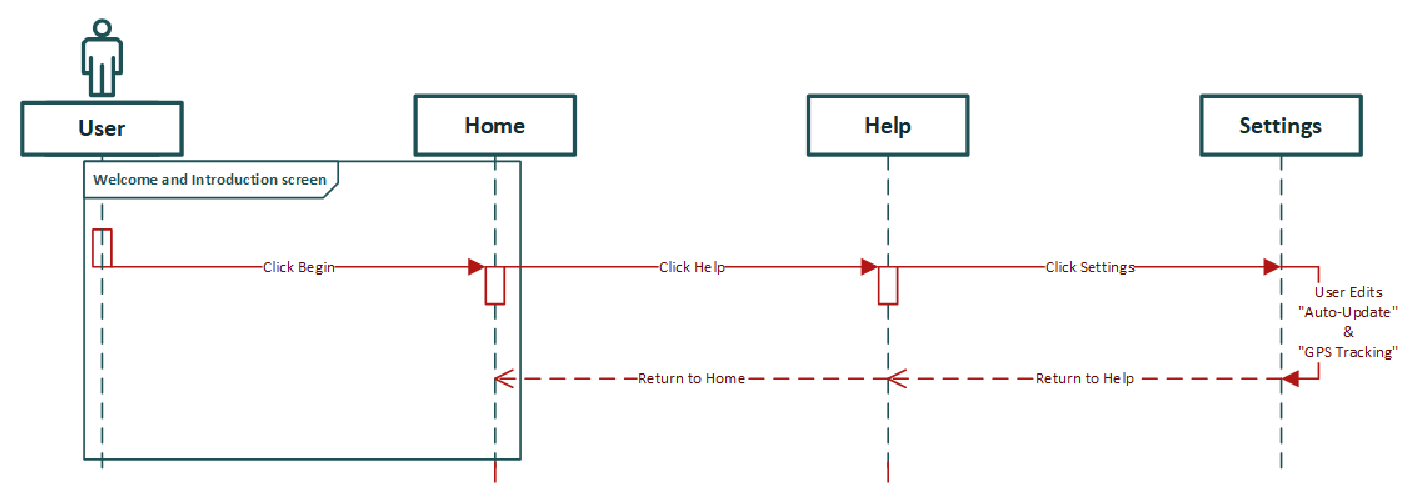
\includegraphics[scale=.7]{Story5.eps}\end{center}
This is the sequence diagram for our "Settings" implementation. It allows the user to alter their settings for the app, including "Auto Update" and "GPS Tracking" settings.
\subsection{Story 6}
\begin{center}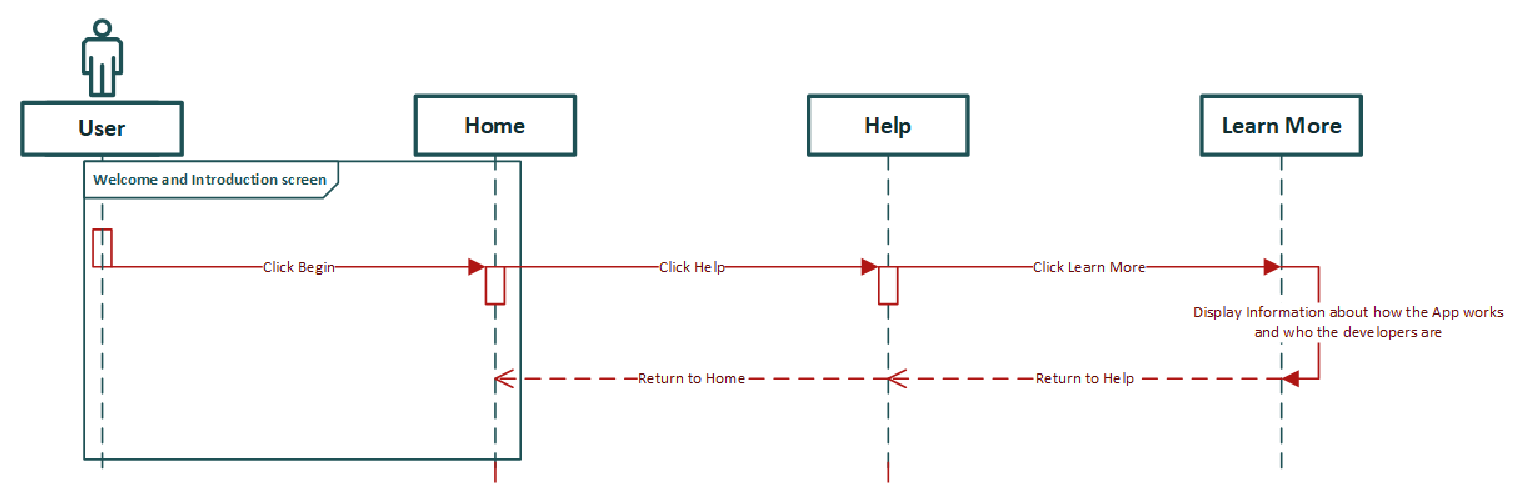
\includegraphics[scale=.65]{Story6.eps}\end{center}
This is the sequence diagram for our "Learn More" implementation. It will display a page explaining the implementation of our app, as well as some information about the developers.
\pagebreak
\subsection{Story 7}
\begin{center}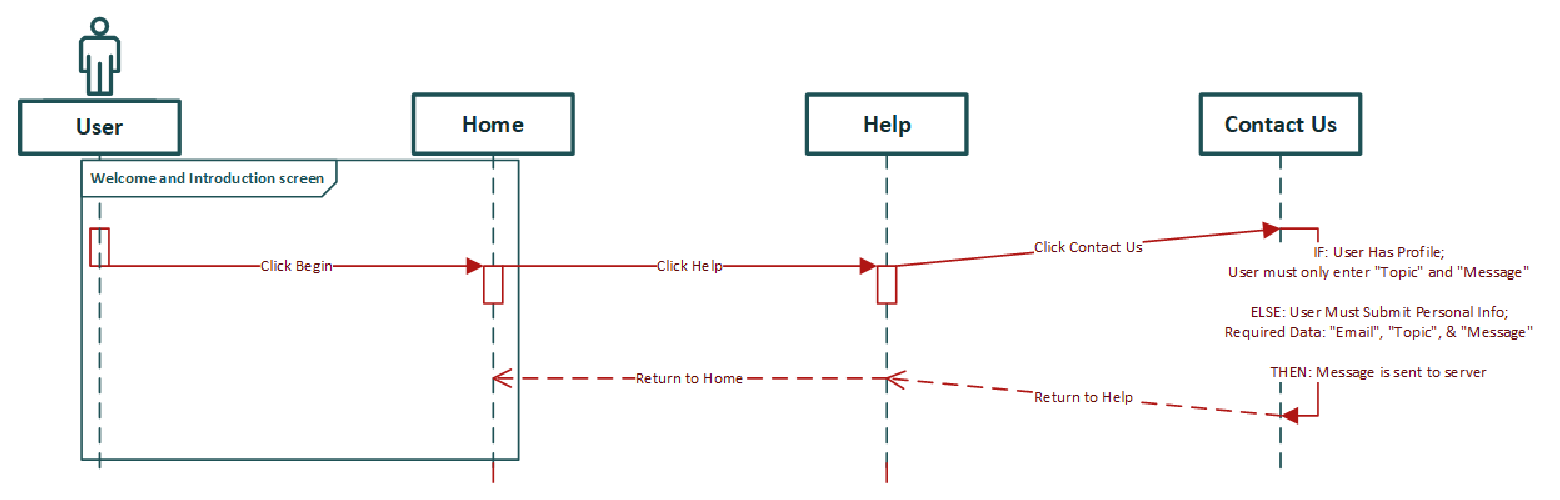
\includegraphics[scale=.65]{Story7.eps}\end{center}
This is the sequence diagram for our "Contact Us" implementation. It allows the user to send feedback or questions about the app to the developers. If they have an account, it will automatically include their email for developers to respond at. If they do not, they will need to enter their email. This information will be stored securely on our database
\subsection{Story 10}
\begin{center}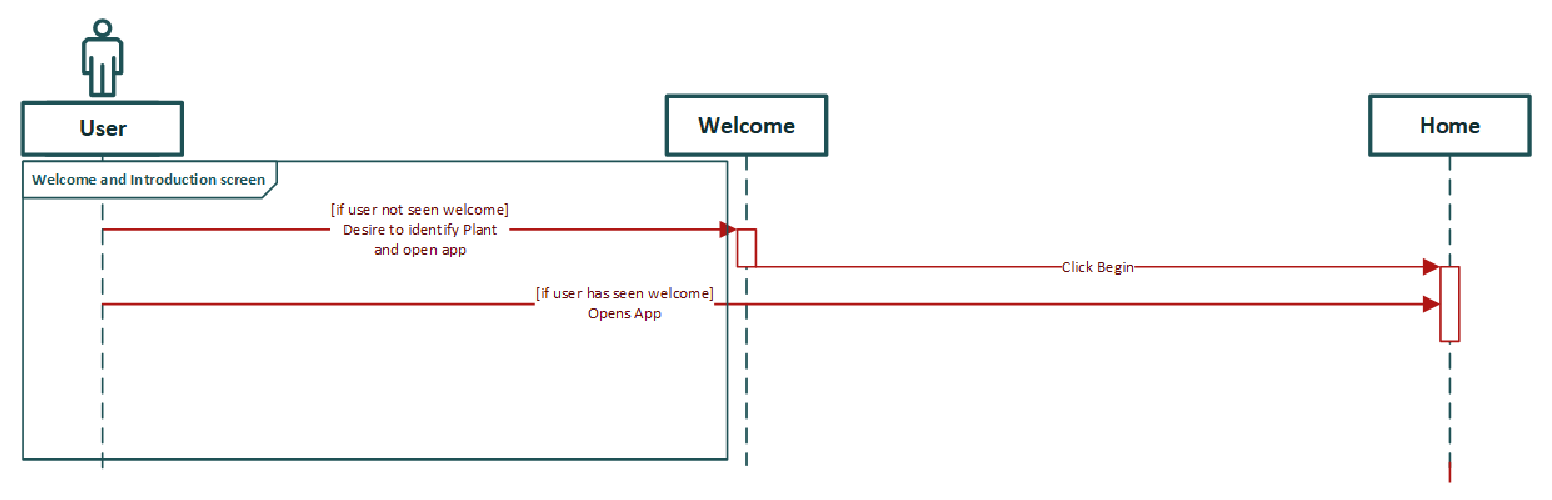
\includegraphics[scale=.65]{Story10.eps}\end{center}
This is the implementation for our "Welcome Page" implementation. It will display a simple welcome message when the user first opens the application after download, explaining how the app works.

\pagebreak
\section{Stories Due Next Week}
Next week we will implement stories 1, 3, and 4. We will be working on implementing story 1 over the next two weeks, since it is the most complex part of our implementation.

\subsection{Story 1 - 20 Questions}

There are two aspects to implementing this story. First, we need to set up a small database to test our implementation with along the way. We will put together a simple dataset of about 100 plants and then construct our binary search tree for them. The other part of the implementation is the 20 questions system that navigates the tree. We've gone into an extensive explanation of how we will implement this in previous assignments, but will include it here again. 

Our implementation will store all of the plant information in a tree data structure, with each node containing a question and each leaf (node with no branches coming off of it) containing a plant. This allows us to simplistically navigate down the tree based on the user's answers to questions. This means we will store a local version of this tree on the user's app and push updates to it when appropriate. The nodes will store pointers to question and plant objects, allowing us to easily edit the questions and plants without altering the structure of the tree. A possible risk with this is a failure to implement pushing updates to the local tree, as none of us are familiar with this process. However, an alternative would be to push updates to the app on the Google Play Store, which users would then download to update their local tree. This is less convenient, but accomplishes the same goal.

We will progress piece by piece on this story at each of our meetings, which will include the dates mentioned in section 4 of this document, as well as further unplanned meetings. 

\subsection{Story 3 - Incorrect Identification}

This story is an error catching feature for Story 1. It allows the user to report when the identification system incorrectly identifies a plant. They can send a report that the identification was incorrect, along with a photo of the plant if they choose. We may not be able to implement the photo sending feature, depending on time constraints. The implementation will simply be adding an entry to the SQL database for administrators to review. Note that Story 13 complements this story, allowing users to submit their feedback while offline. 

\subsection{Story 4 - Correct Identification}

This story displays information about the identified plant to the user. This includes the plant's name, its edibility, if it is safe to touch, and images of the plant pulled from a Google search if the user is connected to the internet. Implementation of this will be simple, pulling information from the relevant Plant object and printing it to the screen.

\pagebreak
\section{Other Stories}
\begin{itemize}
\item Story 2: Image  Identification | Story 2 was originally part of the core design of the app but due to time constraints developing a neural network it out of the question. We could implement, taking pictures of trees for fun, but it would not be accurate. 
\item Story 8: Creating an Account | The account system would let a user add their Name and image to a profile that holds their account activity such as plants found and geotags placed. Its superfluous to the core implementation of the app, so we will likely not include it.
\item Story 9: Become A Botanist | This system would allow a botanist to submit information about themselves that would allow us to verify that they are who they say they are. Again, due to time constraints, this seems out of the question. Formalities related to identifying a certified botanist 
\item Story 11: Reward System |
The reward system is completely superfluous but it would be fun! The app would have achievements awarded for doing things like "Identify 10 Plants" or "Login 3 Days in a row!" Silly things that would make the experience more "whole" as an app. If possible it would be linked through the Google Play Store as they have a system for awarding points for in app achievements. As this has very little to do with the core design of the app, it will most likely be left behind.   
\item Story 12: Social Media | Everything's connected, so why shouldn't your plants be? Similar to the reward system, this is very superfluous and will likely be abandoned in favor of improving our core implementation.

These Stories are Very Hard
\end{itemize}
\section{Meeting Report}
\textbf{02/24/2018 (2:00pm - 6:00pm):} Johnson Hall - Room 219
\begin{itemize}
\item Ethan A, Ethan P, James, and Evan all met to work on this assignment. We also laid out our plan for the coming weeks.
\item We will meet again on 2/28/2018 and 3/3/2018 to work on our implementation, focusing on the stories laid out in our section 4 of this document. We will also begin working on the stories from section 5
\end{itemize}
\end{document}
